 \documentclass[12pt,a4paper]{article}
\usepackage{hyperref} % Use the Charter font for the document text
%\usepackage[UTF8]{ctex}
\usepackage{fullpage}
\usepackage{amsfonts,amssymb,amsmath}
\usepackage{mathtools}
\usepackage{tikz-cd}
\usepackage{tikz}

\usepackage{alltt}
\usepackage{amsfonts}
\usepackage{amsmath}
\usepackage{amssymb}
\usepackage{amsthm}
\usepackage{booktabs}
\usepackage{caption}
\usepackage{enumitem}
\usepackage{fancyhdr}
\usepackage{graphicx}
\usepackage{mathdots}
\usepackage{mathtools}
\usepackage{microtype}
\usepackage{multirow}
\usepackage{pdflscape}
\usepackage{pgfplots}
\usepackage{siunitx}
\usepackage{slashed}
\usepackage{tabularx}
\usepackage{tikz}
\usepackage{tkz-euclide}
\usepackage[normalem]{ulem}
\usepackage[all]{xy}
\usepackage{imakeidx}

\newcommand{\bA}{\ensuremath{\mathbb{A}}}
\newcommand{\bB}{\ensuremath{\mathbb{B}}}
\newcommand{\bC}{\ensuremath{\mathbb{C}}}
\newcommand{\bD}{\ensuremath{\mathbb{D}}}
\newcommand{\bE}{\ensuremath{\mathbb{E}}}
\newcommand{\bF}{\ensuremath{\mathbb{F}}}
\newcommand{\bG}{\ensuremath{\mathbb{G}}}
\newcommand{\bH}{\ensuremath{\mathbb{H}}}
\newcommand{\bI}{\ensuremath{\mathbb{I}}}
\newcommand{\bJ}{\ensuremath{\mathbb{J}}}
\newcommand{\bK}{\ensuremath{\mathbb{K}}}
\newcommand{\bL}{\ensuremath{\mathbb{L}}}
\newcommand{\bM}{\ensuremath{\mathbb{M}}}
\newcommand{\bN}{\ensuremath{\mathbb{N}}}
\newcommand{\bO}{\ensuremath{\mathbb{O}}}
\newcommand{\bP}{\ensuremath{\mathbb{P}}}
\newcommand{\bQ}{\ensuremath{\mathbb{Q}}}
\newcommand{\bR}{\ensuremath{\mathbb{R}}}
\newcommand{\bS}{\ensuremath{\mathbb{S}}}
\newcommand{\bT}{\ensuremath{\mathbb{T}}}
\newcommand{\bU}{\ensuremath{\mathbb{U}}}
\newcommand{\bV}{\ensuremath{\mathbb{V}}}
\newcommand{\bW}{\ensuremath{\mathbb{W}}}
\newcommand{\bX}{\ensuremath{\mathbb{X}}}
\newcommand{\bY}{\ensuremath{\mathbb{Y}}}
\newcommand{\bZ}{\ensuremath{\mathbb{Z}}}


%
%\parskip=1em
%\parindent=0.3in
%\setlength\oddsidemargin{0.5in} \setlength\evensidemargin{0.5in}
%\setlength\textwidth{5.5in}
%
%\hfuzz6pt % Don't bother to report over-full boxes if over-edge is < 6pt
%
%\newlength{\defbaselineskip}
%\setlength{\defbaselineskip}{\baselineskip}
%\newcommand{\setlinespacing}[1]%
%           {\setlength{\baselineskip}{#1 \defbaselineskip}}
%\newcommand{\doublespacing}{\setlength{\baselineskip}%
%                           {2.0 \defbaselineskip}}
%\newcommand{\singlespacing}{\setlength{\baselineskip}{\defbaselineskip}}
%
%\newcommand{\properpagestyle}{\pagestyle{myheadings}\markboth{}{}\markright{}}




\def\Ric{\mathop{\rm Ric}}
\def\cRic{\mathop{\stackrel{\circ}{\Ric}}}
\def\Scal{\mathop{\rm R}}
\def\scL{\mathop{\mathcal L}}
\def\Hess{\mathop{\rm Hess}}
\def\bt{\mathop{\bar\tau}}
\def\dist{\mathop{\rm dist}}
\def\Cut{\mathop{\rm Cut}}
\def\Riem{\mathop{\rm Rm}}
\def\scal{\mathop{\rm scal}}
\def\Sec{\mathop{\rm Sec}}
\def\Diam{\mathop{\rm Diam}}
\def\CS{\mathop{\rm C_S}}
\def\V{\mathop{\rm V}}
\def\Vol{\mathop{\rm Vol}}
\def\Area{\mathop{\rm Area}}
\def\VR{\mathop{\rm VR}}
\def\supp{\mathop{\rm supp}}
\def\div{\mathop{\rm div}}
\def\inj{\mathop{\rm inj}}
\def\diam{\mathop{\rm diam}}
\def\Id{\mathop{\rm Id}}
\def\RRR{\mathop{\mathcal{R}}}
\def\MMM{\mathop{\mathcal{M}}}
\def\HHH{\mathop{\mathcal{H}}}
\def\VVV{\mathop{\mathcal{V}}}
\def\FF{\mathop{\mathbb{F}}}
\def\RR{\mathop{\mathbb{R}}}
\def\QQ{\mathop{\mathbb{Q}}}
\def\CC{\mathop{\mathbb{C}}}
\def\ZZ{\mathop{\mathbb{Z}}}
\def\SS{\mathop{\mathbb{S}}}
\def\SSS{\mathop{\mathcal{S}}}
\def\PP{\mathop{\mathbb{P}}}
\def\End{\mathop{\rm End}}
\def\Aut{\mathop{\rm Aut}}
\def\Ad{\mathop{\rm Ad}}
\def\ad{\mathop{\rm ad}}
\def\hht{\mathop{\rm ht}}
\def\gl{\mathop{\mathfrak{gl}}}
\def\ssl{\mathop{\mathfrak{sl}}}
\def\TP{\mathop{\mathcal{TP}}}
\def\PPP{\mathop{\mathcal{P}}}
\def\gggg{\mathop{\mathfrak{g}}}
\def\ffff{\mathop{\mathfrak{f}}}
\def\OO{\mathop{\mathcal{O}}}
\def\oo{\mathop{\mathfrak{o}}}
\def\GG{\mathop{\mathcal{G}}}
\def\WWW{\mathop{\mathcal{W}}}
\def\Rad{\mathop{\rm Rad}}
\def\Der{\mathop{\rm Der}}
\def\Ker{\mathop{\rm Ker}}
\def\Im{\mathop{\rm Im}}

\def\be{\begin{eqnarray}}
\def\ee{\end{eqnarray}}
\def\beg{\begin{eqnarray*}}
\def\ees{\end{eqnarray*}}


%\newcommand{\qed}{\hfill$\Box$}
\theoremstyle{definition}
\newtheorem*{aim}{Aim}
\newtheorem*{axiom}{Axiom}
\newtheorem*{claim}{Claim}
\newtheorem*{cor}{Corollary}
\newtheorem*{conjecture}{Conjecture}
\newtheorem*{defi}{Definition}
\newtheorem*{eg}{Example}
\newtheorem*{ex}{Exercise}
\newtheorem*{fact}{Fact}
\newtheorem*{law}{Law}
\newtheorem*{lemma}{Lemma}
\newtheorem*{notation}{Notation}
\newtheorem*{prop}{Proposition}
\newtheorem*{question}{Question}
\newtheorem*{thm}{Theorem}





% Maths symbols
\newcommand{\abs}[1]{\left\lvert #1\right\rvert}
%\newcommand\ad{\mathrm{ad}}
\newcommand\AND{\mathsf{AND}}
\newcommand\Art{\mathrm{Art}}
\newcommand{\Bilin}{\mathrm{Bilin}}
\newcommand{\bket}[1]{\left\lvert #1\right\rangle}
\newcommand{\B}{\mathcal{B}}
\newcommand{\bolds}[1]{{\bfseries #1}}
\newcommand{\brak}[1]{\left\langle #1 \right\rvert}
\newcommand{\braket}[2]{\left\langle #1\middle\vert #2 \right\rangle}
\newcommand{\bra}{\langle}
\newcommand{\cat}[1]{\mathsf{#1}}
\newcommand{\C}{\mathbb{C}}
\newcommand{\cU}{\mathcal{U}}
%\newcommand{\Der}{\mathrm{Der}}
\newcommand{\D}{\mathrm{D}}
\newcommand{\dR}{\mathrm{dR}}
\newcommand{\E}{\mathbb{E}}
\newcommand{\F}{\mathbb{F}}
\newcommand{\Frob}{\mathrm{Frob}}
%\newcommand{\GG}{\mathbb{G}}
%\newcommand{\gl}{\mathfrak{gl}}
\newcommand{\GL}{\mathrm{GL}}
\newcommand{\G}{\mathcal{G}}
\newcommand{\Gr}{\mathrm{Gr}}
\newcommand{\haut}{\mathrm{ht}}
\newcommand{\Hol}{\mathrm{Hol}}
\newcommand{\hol}{\mathfrak{hol}}
%\newcommand{\Id}{\mathrm{Id}}
\newcommand{\ket}{\rangle}
\newcommand{\lie}[1]{\mathfrak{#1}}
\newcommand{\Mat}{\mathrm{Mat}}
\newcommand{\N}{\mathbb{N}}
\newcommand{\norm}[1]{\left\lVert #1\right\rVert}
\newcommand{\normalorder}[1]{\mathop{:}\nolimits\!#1\!\mathop{:}\nolimits}
\newcommand{\NOT}{\mathsf{NOT}}
\newcommand{\op}{\mathrm{op}}
\newcommand{\Oc}{\mathcal{O}}
\newcommand{\Or}{\mathrm{O}}
\newcommand\OR{\mathsf{OR}}
\newcommand{\ort}{\mathfrak{o}}
\newcommand{\PGL}{\mathrm{PGL}}
\newcommand{\ph}{\,\cdot\,}
\newcommand{\pr}{\mathrm{pr}}
\newcommand{\Prob}{\mathbb{P}}
\newcommand{\PSL}{\mathrm{PSL}}
\newcommand{\Ps}{\mathcal{P}}
\newcommand{\PSU}{\mathrm{PSU}}
\newcommand{\pt}{\mathrm{pt}}
\newcommand{\qeq}{\mathrel{``{=}"}}
\newcommand{\Q}{\mathbb{Q}}
\newcommand{\R}{\mathbb{R}}
\newcommand{\Rs}{\mathcal{R}}
\newcommand{\SL}{\mathrm{SL}}
\newcommand{\so}{\mathfrak{so}}
\newcommand{\SO}{\mathrm{SO}}
\newcommand{\Spin}{\mathrm{Spin}}
\newcommand{\Sp}{\mathrm{Sp}}
\newcommand{\su}{\mathfrak{su}}
\newcommand{\SU}{\mathrm{SU}}
\newcommand{\term}[1]{\textbf{#1}\index{#1}}
\newcommand{\T}{\mathbb{T}}
\newcommand{\tv}[1]{|#1|}
\newcommand{\U}{\mathrm{U}}
\newcommand{\uu}{\mathfrak{u}}
\newcommand{\Vect}{\mathrm{Vect}}
\newcommand{\wsto}{\stackrel{\mathrm{w}^*}{\to}}
\newcommand{\wt}{\mathrm{wt}}
\newcommand{\wto}{\stackrel{\mathrm{w}}{\to}}
\newcommand{\Z}{\mathbb{Z}}
\renewcommand{\d}{\mathrm{d}}
\renewcommand{\H}{\mathbb{H}}
\renewcommand{\P}{\mathbb{P}}
\renewcommand{\sl}{\mathfrak{sl}}
\renewcommand{\vec}[1]{\boldsymbol{\mathbf{#1}}}
%\renewcommand{\F}{\mathcal{F}}

\let\Im\relax
\let\Re\relax

\DeclareMathOperator{\adj}{adj}
\DeclareMathOperator{\Ann}{Ann}
\DeclareMathOperator{\area}{area}
%\DeclareMathOperator{\Aut}{Aut}
\DeclareMathOperator{\Bernoulli}{Bernoulli}
\DeclareMathOperator{\betaD}{beta}
\DeclareMathOperator{\bias}{bias}
\DeclareMathOperator{\binomial}{binomial}
\DeclareMathOperator{\card}{card}
\DeclareMathOperator{\ccl}{ccl}
\DeclareMathOperator{\Char}{char}
\DeclareMathOperator{\ch}{ch}
\DeclareMathOperator{\cl}{cl}
\DeclareMathOperator{\cls}{\overline{\mathrm{span}}}
\DeclareMathOperator{\coker}{coker}
\DeclareMathOperator{\conv}{conv}
\DeclareMathOperator{\corr}{corr}
\DeclareMathOperator{\cosec}{cosec}
\DeclareMathOperator{\cosech}{cosech}
\DeclareMathOperator{\cov}{cov}
\DeclareMathOperator{\covol}{covol}
\DeclareMathOperator{\diag}{diag}
%\DeclareMathOperator{\diam}{diam}
\DeclareMathOperator{\Diff}{Diff}
\DeclareMathOperator{\disc}{disc}
\DeclareMathOperator{\dom}{dom}
%\DeclareMathOperator{\End}{End}
\DeclareMathOperator{\energy}{energy}
\DeclareMathOperator{\erfc}{erfc}
\DeclareMathOperator{\erf}{erf}
\DeclareMathOperator*{\esssup}{ess\,sup}
\DeclareMathOperator{\ev}{ev}
\DeclareMathOperator{\Ext}{Ext}
\DeclareMathOperator{\fst}{fst}
\DeclareMathOperator{\Fit}{Fit}
\DeclareMathOperator{\fix}{fix}
\DeclareMathOperator{\Frac}{Frac}
\DeclareMathOperator{\Gal}{Gal}
\DeclareMathOperator{\gammaD}{gamma}
\DeclareMathOperator{\gr}{gr}
\DeclareMathOperator{\hcf}{hcf}
\DeclareMathOperator{\Hom}{Hom}
\DeclareMathOperator{\id}{id}
\DeclareMathOperator{\Image}{image}
\DeclareMathOperator{\Im}{Im}
\DeclareMathOperator{\Ind}{Ind}
\DeclareMathOperator{\Int}{Int}
\DeclareMathOperator{\Isom}{Isom}
\DeclareMathOperator{\lcm}{lcm}
\DeclareMathOperator{\length}{length}
\DeclareMathOperator{\Lie}{Lie}
\DeclareMathOperator{\like}{like}
\DeclareMathOperator{\Lk}{Lk}
\DeclareMathOperator{\Maps}{Maps}
\DeclareMathOperator{\mse}{mse}
\DeclareMathOperator{\multinomial}{multinomial}
\DeclareMathOperator{\orb}{orb}
\DeclareMathOperator{\ord}{ord}
\DeclareMathOperator{\otp}{otp}
\DeclareMathOperator{\Poisson}{Poisson}
\DeclareMathOperator{\poly}{poly}
\DeclareMathOperator{\rank}{rank}
\DeclareMathOperator{\rel}{rel}
%\DeclareMathOperator{\Rad}{Rad}
\DeclareMathOperator{\Re}{Re}
\DeclareMathOperator*{\res}{res}
\DeclareMathOperator{\Res}{Res}
%\DeclareMathOperator{\Ric}{Ric}
\DeclareMathOperator{\rk}{rk}
\DeclareMathOperator{\Rees}{Rees}
\DeclareMathOperator{\Root}{Root}
\DeclareMathOperator{\sech}{sech}
\DeclareMathOperator{\sgn}{sgn}
\DeclareMathOperator{\snd}{snd}
\DeclareMathOperator{\Spec}{Spec}
\DeclareMathOperator{\spn}{span}
\DeclareMathOperator{\stab}{stab}
\DeclareMathOperator{\St}{St}
%\DeclareMathOperator{\supp}{supp}
\DeclareMathOperator{\Syl}{Syl}
\DeclareMathOperator{\Sym}{Sym}
\DeclareMathOperator{\tr}{tr}
\DeclareMathOperator{\Tr}{Tr}
\DeclareMathOperator{\var}{var}
\DeclareMathOperator{\vol}{vol}
\usetikzlibrary{knots}

\def\CY{Calabi--Yau}
\def\CP{\mathbb{C}\mathbf{P}}
\def\RP{\mathbb{R}\mathbf{P}}



\pgfarrowsdeclarecombine{twolatex'}{twolatex'}{latex'}{latex'}{latex'}{latex'}
\tikzset{->/.style = {decoration={markings,
                                  mark=at position 1 with {\arrow[scale=2]{latex'}}},
                      postaction={decorate}}}
\tikzset{<-/.style = {decoration={markings,
                                  mark=at position 0 with {\arrowreversed[scale=2]{latex'}}},
                      postaction={decorate}}}
\tikzset{<->/.style = {decoration={markings,
                                   mark=at position 0 with {\arrowreversed[scale=2]{latex'}},
                                   mark=at position 1 with {\arrow[scale=2]{latex'}}},
                       postaction={decorate}}}
\tikzset{->-/.style = {decoration={markings,
                                   mark=at position #1 with {\arrow[scale=2]{latex'}}},
                       postaction={decorate}}}
\tikzset{-<-/.style = {decoration={markings,
                                   mark=at position #1 with {\arrowreversed[scale=2]{latex'}}},
                       postaction={decorate}}}
\tikzset{->>/.style = {decoration={markings,
                                  mark=at position 1 with {\arrow[scale=2]{latex'}}},
                      postaction={decorate}}}
\tikzset{<<-/.style = {decoration={markings,
                                  mark=at position 0 with {\arrowreversed[scale=2]{twolatex'}}},
                      postaction={decorate}}}
\tikzset{<<->>/.style = {decoration={markings,
                                   mark=at position 0 with {\arrowreversed[scale=2]{twolatex'}},
                                   mark=at position 1 with {\arrow[scale=2]{twolatex'}}},
                       postaction={decorate}}}
\tikzset{->>-/.style = {decoration={markings,
                                   mark=at position #1 with {\arrow[scale=2]{twolatex'}}},
                       postaction={decorate}}}
\tikzset{-<<-/.style = {decoration={markings,
                                   mark=at position #1 with {\arrowreversed[scale=2]{twolatex'}}},
                       postaction={decorate}}}


\tikzset{circ/.style = {fill, circle, inner sep = 0, minimum size = 3}}
\tikzset{scirc/.style = {fill, circle, inner sep = 0, minimum size = 1.5}}
\tikzset{mstate/.style={circle, draw, blue, text=black, minimum width=0.7cm}}

\tikzset{eqpic/.style={baseline={([yshift=-.5ex]current bounding box.center)}}}
\tikzset{commutative diagrams/.cd,cdmap/.style={/tikz/column 1/.append style={anchor=base east},/tikz/column 2/.append style={anchor=base west},row sep=tiny}}


\definecolor{mblue}{rgb}{0.2, 0.3, 0.8}
\definecolor{morange}{rgb}{1, 0.5, 0}
\definecolor{mgreen}{rgb}{0.1, 0.4, 0.2}
\definecolor{mred}{rgb}{0.5, 0, 0}


%\title{ Lecture 4}
\begin{document}\thispagestyle{empty}

\centerline{\Large \bf Extra Lecture 2}

\section{Symplectic geometry}


A symplectic form on a smooth manifold $M$ is non-degenerate closed 2-form $\omega$. ``Non-degenerate'' means that the mapping $\omega : TM \to T^*M$; $X \mapsto \omega(X,-)$
 is an isomorphism. We denote the 1-form $\omega(X,-)$ by $i(X)\omega$.
 
 
 The couple ($M, \omega$) of a smooth manifold $M$ and a symplectic form $\omega$ is called a
\term{symplectic manifold}. Any symplectic manifold is even dimensional and if dim($M) =
2n$, $\omega^n$ is a volume-form. 
 
 
 \begin{eg}
 Let $(q_1,\cdots, q_n,p_1,\cdots, p_n)$ be the standard coordinate of $\R^{2n}$. Then,
 $$
\omega=\sum_{i=1}^n dq_i\wedge dp_i~
 $$
 is the symplectic form.
 \end{eg}
 
  \begin{eg}[cotangent bundle]
A symplectic manifold $(M,\omega)$ is called \term{exact} if there exists one form $\theta$ such that $\omega=d\theta$ where $\theta$ is called \term{Liouville 1-form}. The  vector field $Z$ dual to the Liouville 1-form with respect to $\omega$
$$
i_Z\omega=\theta
$$
is called  \term{Liouville vector field}. The most important example of exact symplectic manifolds is a cotengent bundle $M=T^*N$ of a smooth manifold $N$. Given a local coordinate $(q_1,\cdots,q_n)$, they induces the coordinate $(p_1,\cdots,p_n)$ on the fiber $T^*_qN$. Then, the Liouville 1-form is written in terms of the local coordinate of $T^*N$
$$
\theta=\sum_{i=1}^np_id q_i
$$
so that the symplectic form can be locally written as
$$
\omega=\sum_{i=1}^n dq_i\wedge dp_i~.
$$
 \end{eg}
 
 \begin{eg}
 A K\"ahler manifold is a symplectic manifold $(M,\omega)$ equipped with an integrable almost-complex structure $J$ which is compatible with the symplectic form $\omega$, meaning that the bilinear form
$$g(u,v)=\omega (u,Jv)$$
on the tangent space of $M$ at each point is symmetric and positive definite (and hence a Riemannian metric on $M$).
 \end{eg}

 
 
  \begin{thm}[Darboux's theorem]
Let $(M, \omega)$ be a $2n$-dimensional symplectic manifold,
and let $p$ be any point in $M$.
Then there is a coordinate chart $(U, q_1,\cdots , q_n,p_1,\cdots,p_n)$ centered at $p$ such that
on $U$
\be\label{symp}\omega=\sum_{i=1}^n dq_i\wedge dp_i~.\ee
 \end{thm}
 
This theorem states that any symplectic manifold is locally equivalent
to an Euclidean space with its standard symplectic structure. As a result, the most
important questions in symplectic geometry are the global ones.


\subsection{Symplectomorphisms}

 The important maps in symplectic topology are the \term{symplectomorphisms}. A symplectomorphism
between two symplectic manifolds $(M, \omega_M)$ and $(N, \omega_N )$ is a diffeomorphism
$\psi : M\to N$ such that
$$
\psi^\ast \omega_N=\omega_M~.
$$
In fact, this condition is pretty strong. The necessary condition for the existence of symplectomorphisms is $\dim M \le\dim N$.
 
  \begin{eg}[symplectic group]
Let $E = \R^{2n}$ with basis $\{e_1,\cdots ,e_n,f_1,\cdots ,f_n\}$. Then
$$\omega(e_i,e_j ) = 0~,\quad \omega(f_i,f_j ) = 0~,\quad \omega(e_i
,f_j ) = \delta_{i,j}~ .$$
defines a symplectic structure on $E$. Then,  examples of symplectomorphisms are
$$
Sp(E,\omega)=\{g\in GL(2n,\R) ~|g^TJg=J ~, \quad J=\begin{pmatrix}0&I_n\\-I_N&0\end{pmatrix}\}
$$
which is called the \term{symplectic group}.
 \end{eg}
 
 
 
  \begin{thm}[Moser Stability Theorem] Let $(M, \omega_t)$ be a closed manifold with a family of
cohomologous symplectic forms. Then there is a family of symplectomorphisms $\psi_t
: M \to M$
such that
$$\psi_0 = 1~, \psi^*_t \omega_t = \omega_0~.$$
Moreover, if $\omega_t (q) = \omega_0 (q)$ for all points $q$ on a compact submanifold $Q$ of $M$, we may
assume $\psi_t$ is the identity on $Q$.
 \end{thm}
 
 
This theorem says that one cannot change the symplectic form in any important
way by deforming it, provided that the cohomology class is unchanged. 
 
 \subsection{Lagrangian submanifolds}
 
  \begin{defi}[Lagrangian submanifold]
A Lagrangian submanifold of a sympletic manifold $(M,\omega )$ is a submanifold where the restriction of the symplectic form $\omega$  to $L\subset M$ is vanishing, i.e. $\omega |_{L}=0$ and ${\text{dim }}L=1/2\cdot {\text{dim }}M$. 
\end{defi}

If we perturb a Lagrangian submanifold, then it is no longer Lagrangian in general. Thus, they are ``rigid'' objects in symplectic geometry. Since Lagrangian submanifolds play very important role in symplectic geometry, Weinstein advertised slogan that everything is a Lagrangian submanifold. (A. Weinstein's lagrangian creed.)

  \begin{eg}
The zero section $N$ of the cotangent bundle $M=T^*N$ is a Lagrangian submanifold. Let $f:Z\hookrightarrow N$ is an embedding. Then, the conormal bundle to $Z$ in $T^*N$ defined as
$$L_Z:=\{(x,\alpha)\in T^*N| x\in Z~, \quad \alpha(v)=0~ \textrm{for all}~ v\in T_xZ\}\subset T^*N~,$$
is a Lagrangian submanifold.
\end{eg}

It is known that the neighborhood of a Lagrangian also has the standard symplectic structure as its cotangent bundle.

  \begin{thm}[Weinstein's tubular neighbourhood theorem]
Every lagrangian submanifold $L$ in a symplectic manifold $(M,\omega)$ has a neighbourhood $U$ which is symplectomorphic to a neighbourhood $V$ of the zero section of the cotangent bundle $T^*L$.
\end{thm}

  \subsection{Hamiltonian system}

 Any smooth function $H\in C^\infty(M)$ gives rise to a vector field $X_H$ defined uniquely
by the equation
$$i(X_H)\omega = dH~.$$
This vector field is called the \term{Hamiltonian vector field} with Hamiltonian $H$. Given a symplectic form \eqref{symp},
the flow of the Hamiltonian vector field $X_H$ associated to a Hamiltonian $H$ can be described by 
$$
\frac{dq_i}{dt}=\frac{\partial H}{\partial  p_i}~,\qquad \frac{dp_i}{dt}=-\frac{\partial H}{\partial  q_i}~,
$$
which are Hamilton's canonical equations. 

For $f,g\in C^\infty(M)$, we define the Poisson product by
$$
\{ f,g\}=\omega(X_f,X_g)=X_f(g)=-X_g(f)~.
$$
Given the symplectic form \eqref{symp}, the Poisson product can be written as the local coordinate
 $$
 \{ f,g\}=\sum_{i=1}^n \left(\frac{\partial f}{\partial  q_i}\frac{\partial g}{\partial  p_i}-\frac{\partial f}{\partial  p_i}\frac{\partial g}{\partial  q_i} \right)~.
 $$
 They satisfy the following properties
 \begin{description}
\item{Skew symmetry:} $ \{f,g\}=-\{g,f\}.$
\item{Jacobi identity:} $ \{f,\{g,h\}\}+\{g,\{h,f\}\}+\{h,\{f,g\}\}=0.$
\item{Leibniz's Rule:} $ \{fg,h\}=f\{g,h\}+g\{f,h\}.$
\end{description}
Using these properties, one can show that 
$$
[X_f,X_g]=X_{\{f,g\}}~.
$$
 For $f\in C^\infty(M)$,  the differentiation with respect to the Hamiltonian flow  can be expressed by
 $$
 \frac{df}{dt}=-\{H,f\}~.
 $$
If $\{f,H\}=0$, the flow generated by $X_f$ is a symmetry of the Hamiltonian system with $H$. Namely, if we denote the flow by $\varphi_s$, then we have
$$
\frac{dH}{ds}=\{f,H\}=0~,
$$
 or equivalently, 
 $$
 \frac{df}{dt}=-\{H,f\}=0~.
 $$
This is called \term{Noether theorem.}


\begin{eg}
If they system has spherical symmetry, the potential $V(r)$ is independent of $\theta$ and $\phi$. Then, the momenta $p_\theta$ and $p_\phi$ are conserved.
\end{eg}




 \subsection{Arnold-Liouville theorem}
Let us consider Poisson commuting functions (Hamiltonians)
$H_1, \cdots , H_k$  with $\{H_i, H_j\} = 0$ for all $i, j$. To insure that we are not discussing a degenerate situation, we assume that
$dH_1\wedge \cdots \wedge dH_k(x) \neq 0$ for $\forall x\in M$, in which $H_i$ are called  \term{analytically independent}. Then, the maximal number of Poisson commuting functions is a half of dimension of $M$ which is $n$. An $2n$-dimensional symplectic manifold $(M,\omega)$ with $n$ Poisson commuting Hamiltonians is called \term{completely integrable system}.


\begin{thm}[Arnold-Liouville theorem]
Let $H_1, \cdots , H_n$ be a completely integrable system on a $2n$-dimensional symplectic manifold  $(M,\omega)$. Namely, 
$\pi=(H_1, \cdots , H_n):M\to \R^n$ are analytically independent Poisson commuting functions with $\{H_i, H_j\} = 0$ for all $i, j$. Then, a compact connected component of the preimage of a non-singular point of $\pi$ is a Lagrangian submanifold that is diffeomorphic to a torus $T^n$. 
\end{thm}

Let us denote the image of $\pi$ by $B$. Then, (compact connected component  of) the preimage $L=\pi^{-1}(b)$ of $b\in B$ is diffeomorphic to $T^n$ so that we can take the angle coordinate 
$$
(\phi_1\cdots \phi_n):	L\to T^n
$$
We can further take local coordinate $(I_1,\cdots,I_n)$ of $B$ that the symplectic form can be locally expressed as
$$
\omega=\sum_{i=1}^n d\phi_i\wedge dI_i~,
$$
where $(\phi_i,I_i)$ are called \term{angle-action} coordinate.



\begin{eg}
  Consider the harmonic oscillator with Hamiltonian
  \[
    H(q, p) = \frac{1}{2}p^2 + \frac{1}{2}\omega^2 q^2.
  \]
  Since is a 2-dimensional system, so we only need a single first integral. Since $H$ is a first integral for trivial reasons, this is an integrable Hamiltonian system.

  We can actually draw the lines on which $H$ is constant --- they are just ellipses:
  \begin{center}
    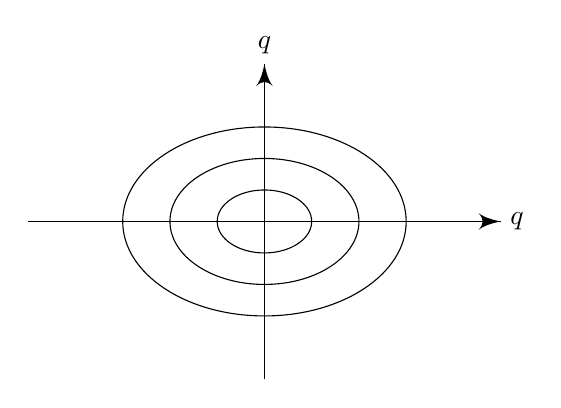
\begin{tikzpicture}
      \draw [->] (-3, 0) -- (3, 0) node [right] {$q$};
      \draw [->] (0, -2) -- (0, 2) node [above] {$q$};

      \foreach \x in {0.4, 0.8, 1.2} {
        \begin{scope}[scale=\x]
          \draw ellipse (1.5 and 1);
        \end{scope}
      }
    \end{tikzpicture}
  \end{center}
  We note that the ellipses are each homeomorphic to $S^1$. Now we introduce the coordinate transformation $(q, p) \mapsto (\phi, I)$, defined by
  \[
    q = \sqrt{\frac{2I}{\omega}} \sin \phi,\quad p = \sqrt{2I\omega} \cos \phi,
  \]
Hence, $\phi$ is the angle coordinate that parametrizes $S^1$ in the Arnold-Liouville theorem.

  We can manually show that this transformation is canonical, but it is merely a computation and we will not waste time doing that. In these new coordinates, the Hamiltonian looks like
  \[
    \tilde{H}(\phi, I) = H(q(\phi, I), p(\phi, I)) = \omega I.
  \]
The Hamiltonian is independent of $\phi$! Therefore, the Hamilton equations become
  \[
    \dot\phi = \frac{\partial \tilde{H}}{ \partial I} = \omega,\quad \dot{I} = -\frac{\partial \tilde{H}}{\partial \phi} = 0.
  \]
  We can integrate up to obtain
  \[
    \phi(t) = \phi_0 + \omega t,\quad I(t) = I_0.
  \]
It is interesting to consider the integral along paths of constant $H$:
  \begin{align*}
    \frac{1}{2\pi}\oint p \;\d q &= \frac{1}{2\pi} \int_0^{2\pi}p(\phi, I) \left(\frac{\partial q}{\partial \phi} \;\d \phi + \frac{\partial q}{\partial I} \;\d I\right)\\
    &= \frac{1}{2\pi} \int_0^{2\pi}p(\phi, I) \left(\frac{\partial q}{\partial \phi} \;\d \phi\right)\\
    &= \frac{1}{2\pi} \int_0^{2\pi} \sqrt{\frac{2I}{\omega}}\sqrt{2I\omega} \cos^2 \phi \;\d \phi\\
    &= I~.
  \end{align*}
We could always have performed the integral $\frac{1}{2\pi} \oint p \;\d q$ along paths of constant $H$ without knowing anything about $I$ and $\phi$, and this would have magically gave us the new coordinate $I$. That's why it is called \term{integrable system}.
\end{eg}












%
%
%\begin{thebibliography}{99}

%\bibitem{Candelas}
%P. Candelas, X. C. de La Ossa, P. S. Green, L. Parkes, \textit{A pair of Calabi-Yau manifolds as an exactly soluble superconformal theory}. Nucl.Phys. B359 (1991) 21-74.
%
%\bibitem{Bouchard}
%Vincent. Bouchard,  \textit{Lectures on complex geometry, Calabi-Yau manifolds and toric geometry.} \href{http://arxiv.org/abs/hep-th/0702063}{hep-th/0702063} (2007).
%
%\bibitem{Calabi-Yau}
%Calabi-Yau manifolds, 
%\url{http://www.scholarpedia.org/article/Calabi-Yau_manifold}
%
%\end{thebibliography}


\end{document}
